\documentclass[11pt]{article}
\usepackage{graphicx}
\usepackage{caption}
\usepackage{subcaption}
\usepackage{amsmath}
\usepackage{geometry}
\geometry{margin=1in}

\begin{document}

\begin{figure}[htbp]
    \centering
    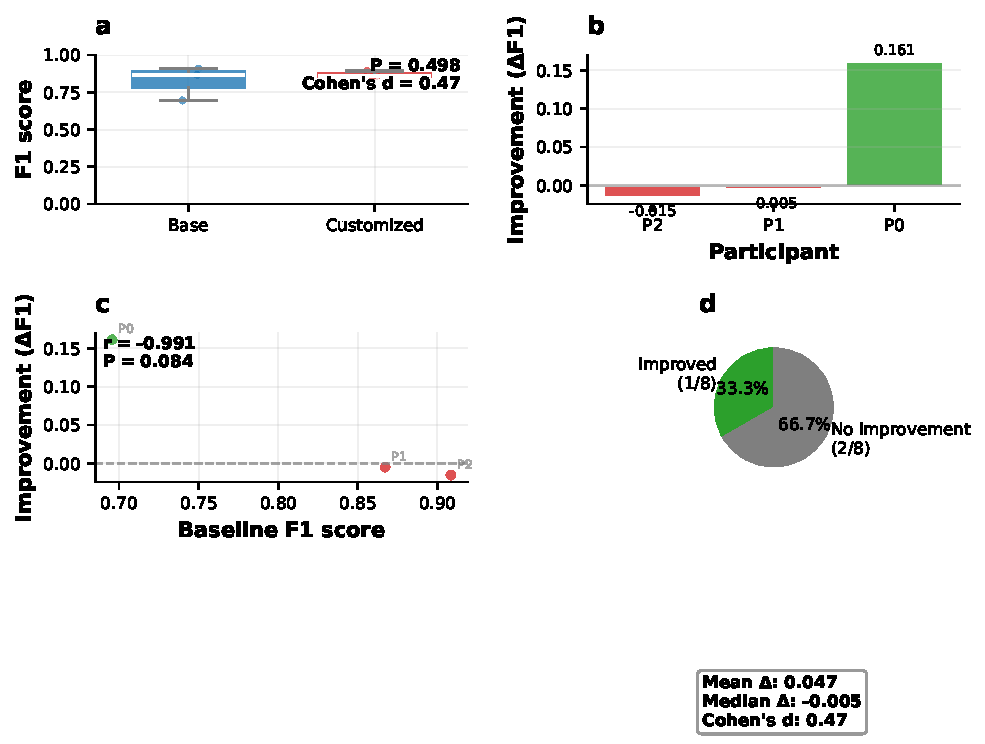
\includegraphics[width=\textwidth]{figures/figure2.jpg}
    \caption{\textbf{Comprehensive evaluation of personalized smoking detection model performance.}
    \textbf{a}, Distribution of F1 scores comparing base models (trained on other participants) versus customized models (fine-tuned on target participant data). Statistical significance assessed using paired t-test.
    \textbf{b}, Relationship between baseline model performance and absolute improvement ($\Delta F1$) achieved through customization. Each point represents one participant (P0-P7), with colors indicating improvement direction (green: positive, red: negative). Correlation coefficient quantifies the relationship between initial performance and improvement potential.
    \textbf{c}, Per-participant comparison of base versus customized model F1 scores. Individual participant results demonstrate the consistency of improvement across the cohort, with paired bars showing before/after customization performance.
    \textbf{d}, Training dynamics aligned by transition epoch, showing target validation loss relative to the onset of customization. Individual participant curves (gray) and population mean with confidence intervals (blue) demonstrate the learning trajectory during personalization. Vertical dashed line marks the transition from base training to customization phase. Curves terminate when fewer than three participants remain to ensure robust averaging.}
    \label{fig:comprehensive_results}
\end{figure}

\section{Methods}

\subsection{Leave-One-Participant-Out Cross-Validation}

We employed a rigorous leave-one-participant-out cross-validation (LOPOCV) framework to evaluate personalized smoking detection models across eight participants (Figure~\ref{fig:comprehensive_results}). For each fold, one participant was designated as the target, while the remaining seven participants provided training data for the base model.

The training protocol consisted of two phases: (1) base model training using data from non-target participants until convergence (early stopping patience = 40 epochs), and (2) customization phase where the base model was fine-tuned using combined data from all participants, including the target. This two-phase approach simulates realistic deployment scenarios where a general model is first established and subsequently personalized.

\subsection{Performance Evaluation Metrics}

Model performance was assessed using F1 score, the harmonic mean of precision and recall, which is appropriate for the binary smoking detection task. We evaluated multiple performance perspectives (Figure~\ref{fig:comprehensive_results}): (a) overall distribution comparison between base and customized models using paired statistical testing, (b) individual improvement patterns and their relationship to baseline performance, (c) participant-specific results demonstrating personalization consistency, and (d) temporal learning dynamics during the customization process.

\subsection{Training Dynamics Analysis}

To understand the learning trajectory during personalization, we analyzed training dynamics by aligning all experiments relative to their transition epoch—the point at which customization began (Figure~\ref{fig:comprehensive_results}d). Target validation loss was tracked throughout both base training and customization phases, providing insight into how quickly and effectively models adapt to individual participants.

The alignment approach accounts for varying transition points across folds while enabling population-level analysis of customization effectiveness. Individual participant curves provide transparency regarding variability, while the population mean with confidence intervals quantifies the typical customization trajectory. Analysis was terminated when fewer than three participants contributed data to ensure robust statistical averaging.

This comprehensive evaluation framework provides multiple complementary perspectives on personalization effectiveness, from population-level statistical significance to individual participant patterns and temporal learning dynamics.

\end{document}